% Build from this folder with: tectonic report.tex
% Numbers come from the notebooks' 2026-11-09 run.
\documentclass[11pt]{article}
\usepackage[margin=1in]{geometry}
\usepackage[T1]{fontenc}
\usepackage{lmodern}
\usepackage{microtype}
\usepackage{graphicx}
\usepackage{booktabs}
\usepackage{tabularx}
\usepackage{caption}
\usepackage{enumitem}
\usepackage{xcolor}
\usepackage[hidelinks]{hyperref}
\graphicspath{{../figures/}}
\captionsetup{font=small,labelfont=bf}
\setlist{itemsep=1pt,topsep=3pt}
\setlength{\parskip}{4pt}
\setlength{\parindent}{0pt}

\begin{document}

% ---------------- Cover page ----------------
\begin{titlepage}
\centering
\vspace*{1.5in}
{\LARGE\bfseries Modeling Firm Recovery Across\\[4pt] Three Market Crashes Using SEC Filings\par}
\vspace{0.5in}
{\large Raaj Banga\par}
\vspace{6pt}
{\large Western Kentucky University\par}
\vspace{6pt}
{November 2026\par}
\vspace{0.8in}
\begin{minipage}{0.82\textwidth}
\small
\textbf{Abstract.} We ask whether a firm's financials before a market crash predict whether its stock recovers, and whether that still holds when the next crash has a different cause. Using SEC filings for every U.S.\ public filer, including firms that later failed, we build 10,513 firm-crash rows across the 2020 COVID-19 crash, the 2022 rate-hike bear market, and the 2025 tariff shock. Within a crash, fundamentals beat a sector-and-size baseline (LightGBM AUC 0.67 to 0.70; the bootstrap confidence interval of the gain excludes zero in every crash). Across crashes, the same models fall to about chance and below the baseline (pooled AUC change $-0.055$, 95\% CI $-0.066$ to $-0.044$). The reason is that signals change sign with the crash's cause: volatile stocks recovered best in 2020 and worst in 2022 and 2025. What predicts recovery depends on what caused the crash.
\end{minipage}
\end{titlepage}

% ---------------- 1. Introduction ----------------
\section{Introduction and motivation}

Crashes hit firms unevenly. After the same market drop, some stocks are back at their old price within months, others never return, and some firms are delisted. Investors and lenders would like to know in advance which firms are resilient, using only what is known before the crash.

Most studies of crash resilience look at one event, usually COVID-19. A trait that predicted recovery in one crash may only reflect that crash's cause. This project tests the question directly: we train models on one crash and test them on another.

\textbf{Research questions.}
\begin{itemize}
  \item \textbf{Prediction:} do pre-crash fundamentals predict recovery better than sector and size alone?
  \item \textbf{Transfer:} how much accuracy is lost when a model meets a crash it was not trained on?
  \item \textbf{Signals:} which predictors hold in every crash, and which are crash-specific? This separation is the project's novel contribution.
  \item \textbf{Archetypes, exceptions, and timing:} do kinds of firms recover differently, which firms defied the model, and how long does recovery take?
\end{itemize}

The three crashes have different causes (Table~\ref{tab:crashes}). COVID-19 was a fast liquidity panic followed by a fast rebound. The 2022 decline was a slow repricing driven by rising interest rates. The 2025 tariff shock was short and shallow.

\begin{table}[h]
\centering\small
\caption{The three crashes (S\&P 500 closing prices from FRED).}
\label{tab:crashes}
\begin{tabular}{lllrrl}
\toprule
Crash & Peak & Trough & Drop & VIX high & Index back at peak \\
\midrule
COVID-19 (2020) & 2020-02-19 & 2020-03-23 & $-33.9\%$ & 83 & about 5 months after the trough \\
Rate hikes (2022) & 2022-01-03 & 2022-10-12 & $-25.4\%$ & 36 & about 15 months \\
Tariffs (2025) & 2025-02-19 & 2025-04-08 & $-18.9\%$ & 52 & under 3 months \\
\bottomrule
\end{tabular}
\end{table}

% ---------------- 2. Literature ----------------
\section{Literature review}

Studies of the COVID-19 crash agree that financial strength mattered. Ramelli and Wagner~\cite{ramelli2020} found that as the virus spread, investors marked down firms with high leverage and little cash. Fahlenbrach, Rageth, and Stulz~\cite{fahlenbrach2021} showed that firms with more cash before the crisis fell less, and Ding et al.~\cite{ding2021} found milder declines for firms with stronger pre-2020 finances. Our 2020 model agrees: cash to assets is its top feature.

These studies each cover a single crash, so they cannot tell whether cash matters in general or only in a liquidity crisis. Machine-learning work on stock returns, such as Gu, Kelly, and Xiu~\cite{gu2020}, finds that predictability exists but is small, and that price-based signals such as momentum and volatility carry much of it. We combine the two lines of work: machine-learning models of firm recovery, tested across crashes with different causes.

% ---------------- 3. Dataset ----------------
\section{Dataset description}

\subsection{Sources}
\begin{itemize}
  \item \textbf{SEC EDGAR XBRL company facts}~\cite{secapi}: financial statements, share counts, industry (SIC) codes, and filing histories for 20,547 filers. Delistings and bankruptcies come from Form 25, Form 15, and 8-K filings.
  \item \textbf{SEC fails-to-deliver files}~\cite{secftd}: 185 files from 2019 to 2026. They list each ticker with its issuer code and a recorded price, so they serve as an independent check on tickers and prices.
  \item \textbf{Daily prices:} Yahoo Finance (through \texttt{yfinance}~\cite{yfinance}) for listed firms, and Tiingo~\cite{tiingo} for firms that have since left the market.
  \item \textbf{FRED}~\cite{fred}: the S\&P 500, VIX, and 10-year Treasury yield, used only to describe each crash.
\end{itemize}
FRED does not carry firm-level data, so prices come from Yahoo and Tiingo and industry codes from the SEC.

\subsection{Building the firm-crash table}
Each row is one firm in one crash. Table~\ref{tab:funnel} shows how many rows survive each step.

\begin{itemize}
  \item \textbf{Universe.} We start from SEC filers before each peak rather than today's stock listings, so firms that later failed stay in. We require a 10-K (which excludes foreign filers on Form 20-F) and remove SPACs and firms without public stock.
  \item \textbf{Tickers.} SEC filings identify firms by an ID (CIK), not a ticker. We use the SEC's current ticker, and for dead firms we match names in the fails files, which also link old tickers to new ones (\texttt{SIVB} to \texttt{SIVBQ}). Tickers get reused, so each ticker must belong to the same issuer, under a name the firm used at the peak. This check found 11 rows priced as a different company (Ambac's old ticker now belongs to Overseas Shipholding).
  \item \textbf{Price check.} Each price series is compared with the fails files' recorded prices around the peak. At least 80\% of dates must agree, allowing for one split. 96.6\% of matched rows end up with a checked price.
  \item \textbf{Filters.} We keep common stock only, with a pre-crash price of at least \$1 before split adjustment, a market value of at least \$10M, and trading on at least 70\% of days in the year before the peak. We also drop 46 business development companies.
  \item \textbf{Price cleaning.} One-day spikes above 50\% that are mostly undone the next day are removed. A missed reverse split is fixed only when SEC share counts confirm it (18 rows).
\end{itemize}

\begin{table}[h]
\centering\small
\caption{Rows kept at each step.}
\label{tab:funnel}
\begin{tabular}{lrrrr}
\toprule
Step & 2020 & 2022 & 2025 & Total \\
\midrule
SEC filers with public stock & 5,095 & 5,077 & 5,119 & 15,291 \\
Ticker matched and checked against the firm's identity & & & & 13,392 \\
Price series checked against SEC fails prices & 4,031 & 4,282 & 4,618 & 12,931 \\
Common stock, $\geq$\$1, $\geq$\$10M, actively traded & 3,216 & 3,599 & 3,744 & 10,559 \\
Final table (business development companies removed) & 3,216 & 3,599 & 3,698 & 10,513 \\
\bottomrule
\end{tabular}
\end{table}

\subsection{Labels}
\begin{itemize}
  \item \textbf{Pre-crash price:} the highest adjusted close in the 30 trading days up to the market peak.
  \item \textbf{Recovered within 12 months} (main label): the stock closes at or above its pre-crash price within 12 months of the market trough. Base rates are 75.6\% (2020), 42.8\% (2022), and 69.2\% (2025).
  \item \textbf{Beat the market} (second label): the firm's return from the peak to 12 months after the trough beats SPY's. A firm that stops trading keeps its last price. Base rates are 47.7\%, 32.0\%, and 38.4\%.
  \item \textbf{Days to recovery} (for survival analysis): capped at 18 months. Only failed firms count as never recovering; acquired and otherwise delisted firms are censored at their last trade.
\end{itemize}

\subsection{Features}
There are 16 features. Twelve come from SEC filings: current ratio, cash, debt, and liabilities to assets, interest coverage, net and operating margin, return on assets, operating cash flow to assets, revenue and asset growth, and log assets. Four come from prices: log market value, 12-month volatility, momentum from 12 months to 1 month before the peak, and beta against SPY. Sector is the SIC division.
\begin{itemize}
  \item \textbf{Point in time.} Only facts filed before the peak are used, so later restatements cannot leak in. Flows are trailing 12 months. An automated test confirms that no fact filed and no price dated after the peak is used.
  \item \textbf{Missing values} are kept as missing with a flag. Some gaps are by design: current ratio and interest coverage are left missing for financial firms, and margins need positive revenue.
  \item \textbf{Firm overlap.} 71\% of rows belong to firms that appear in all three crashes, so all cross-validation folds and bootstrap resamples keep each firm's rows together.
\end{itemize}

% ---------------- 4. Methodology ----------------
\section{Approach and methodology}

\textbf{Models.} We compare a baseline logistic regression that only sees sector and size (log assets, log market value) with three full models: logistic regression, random forest~\cite{breiman2001}, and LightGBM~\cite{ke2017}. Hyperparameters are fixed and regularized, not tuned, and classes are balanced with class weights. Inside each pipeline, fitted on training rows only, ratios are capped at the 1st and 99th percentiles, then missing values are filled with the median.

\textbf{Evaluation design.} We use two settings.
\begin{itemize}
  \item \textbf{Within a crash:} 5-fold cross-validation, stratified by label and grouped by firm.
  \item \textbf{Across crashes:} train on one crash and test on each other crash, and also train on two crashes and test on the third.
\end{itemize}
The main metric is AUC, the probability that the model ranks a random recovering firm above a random non-recovering one (0.5 is chance). We use AUC because base rates range from 43\% to 76\%: always predicting ``recovers'' would score 76\% accuracy in 2020.

\textbf{Statistics.} Each model is compared with the baseline on the same test rows using DeLong tests~\cite{delong1988,sun2014}, with Holm's correction across all 72 comparisons~\cite{holm1979}. Confidence intervals come from a bootstrap that resamples whole firms. Feature importance is the mean absolute SHAP value~\cite{lundberg2017}. A feature counts as \emph{universal} if it ranks in the top 5 in all three crashes with the same sign. We compare importance rankings across crashes with Spearman correlation.

\textbf{Patterns and timing.}
\begin{itemize}
  \item \textbf{Archetypes:} k-means on within-crash percentiles, with $k$ chosen by silhouette among stable solutions, checked against HDBSCAN~\cite{campello2013}.
  \item \textbf{Recovery rules:} FP-Growth association rules~\cite{han2000}.
  \item \textbf{Unusual firms:} Isolation Forest~\cite{liu2008} and LOF~\cite{breunig2000}.
  \item \textbf{Timing:} Kaplan--Meier curves~\cite{kaplan1958} and a Cox model~\cite{cox1972} stratified by crash.
\end{itemize}

% ---------------- 5. Results ----------------
\section{Results and analysis}

\subsection{Within a crash, fundamentals beat the baseline}
Table~\ref{tab:within} shows within-crash AUC. Every full model beats the baseline, by 0.02 to 0.07 for LightGBM. For LightGBM, the bootstrap confidence interval of the gain excludes zero for every crash and both labels, and 16 of the 18 full-model gains are significant after Holm's correction. Random forest and LightGBM perform about the same.

\begin{table}[h]
\centering\small
\caption{Within-crash AUC (5-fold cross-validation grouped by firm).}
\label{tab:within}
\begin{tabular}{lccccccc}
\toprule
& \multicolumn{3}{c}{Recovered in 12 months} && \multicolumn{3}{c}{Beat SPY} \\
\cmidrule{2-4}\cmidrule{6-8}
Model & 2020 & 2022 & 2025 && 2020 & 2022 & 2025 \\
\midrule
Baseline (sector, size) & 0.623 & 0.670 & 0.651 && 0.645 & 0.667 & 0.649 \\
Logistic regression & 0.647 & 0.701 & 0.670 && 0.684 & 0.719 & 0.670 \\
Random forest & \textbf{0.683} & \textbf{0.709} & \textbf{0.676} && 0.708 & 0.730 & \textbf{0.679} \\
LightGBM & 0.678 & 0.703 & 0.674 && \textbf{0.714} & \textbf{0.731} & 0.678 \\
\bottomrule
\end{tabular}
\end{table}

\subsection{Across crashes, the models fall below the baseline}
Figure~\ref{fig:transfer} is the main result. Off the diagonal, LightGBM's AUC falls to between 0.46 and 0.60, and every pair involving 2020 is at or below chance. Only 2022 and 2025 transfer partly to each other (0.58 to 0.60). Pooled over all cross-crash tests, LightGBM trained on the other two crashes scores 0.055 \emph{below} the baseline for recovery (95\% CI $-0.066$ to $-0.044$) and 0.048 below for beating SPY. On average LightGBM loses 0.18 AUC moving from within a crash to across crashes, compared with 0.13 for the baseline. A model trained on past crashes is therefore worse than a simple one on the next crash, not just weaker.

Even the most realistic case, training on 2022 and predicting the later 2025 crash, does not beat the baseline (0.602 vs 0.618, not significant).

\begin{figure}[h]
\centering
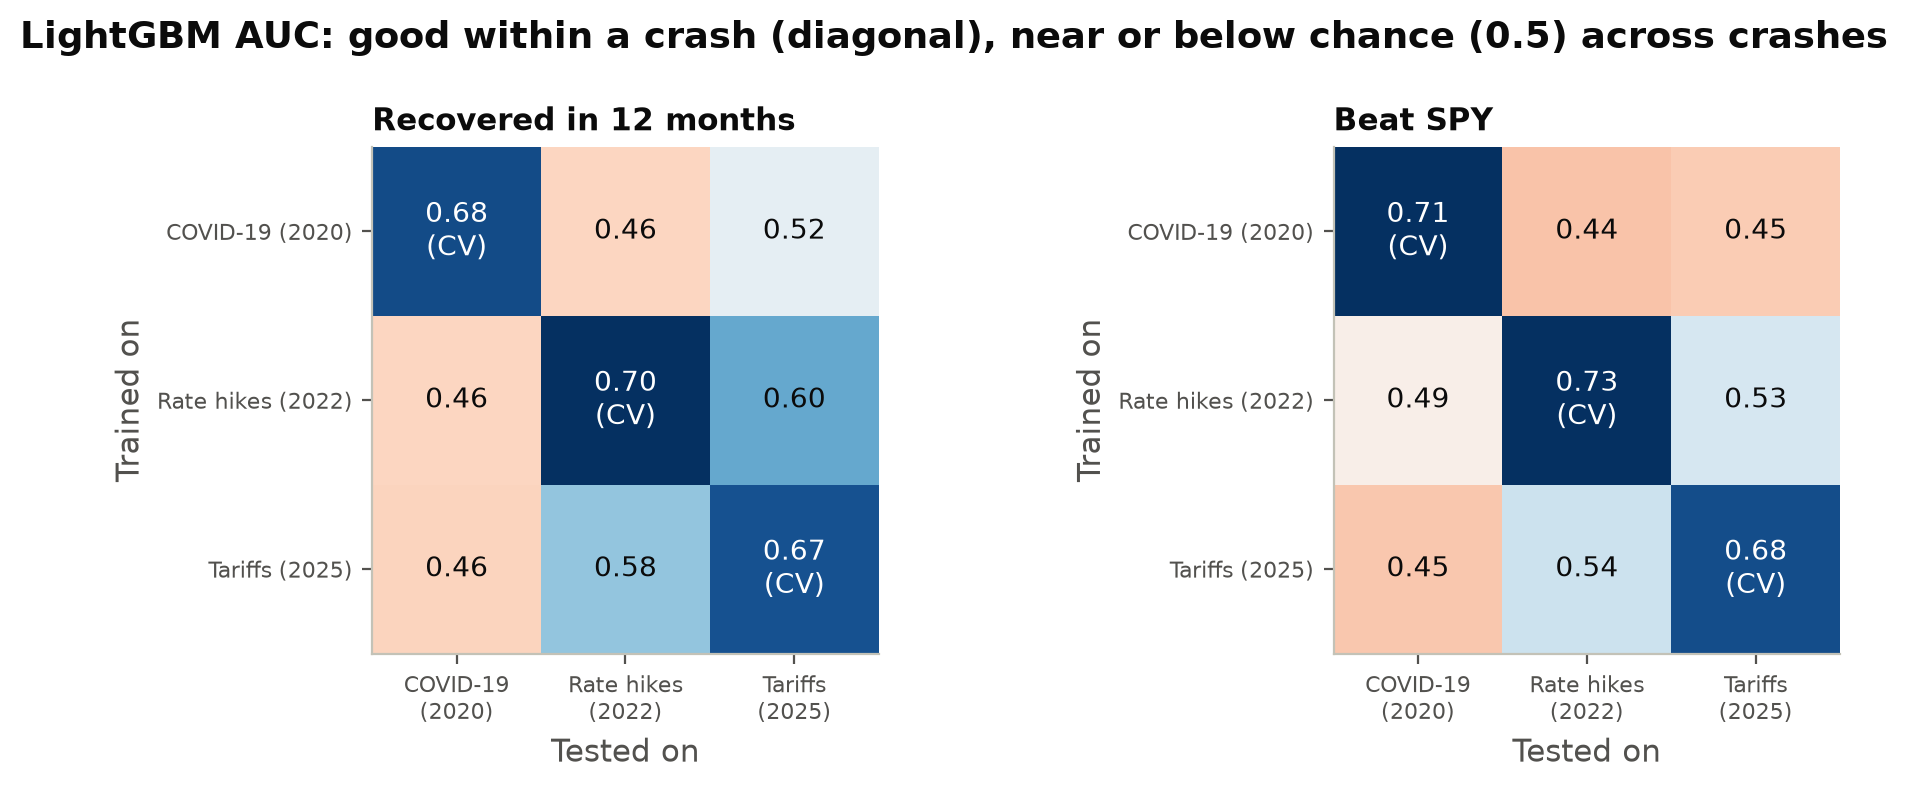
\includegraphics[width=0.88\textwidth]{transfer_auc.png}
\caption{LightGBM AUC by training crash (rows) and test crash (columns). The diagonal is within-crash cross-validation.}
\label{fig:transfer}
\end{figure}

\subsection{Why: signals change sign with the crash}
No feature meets our rule for a universal signal. The closest is log assets, which has the same sign everywhere but ranks only 7th in 2020. Each crash has its own leading signals: cash to assets and market value in 2020, asset growth and momentum in 2022, and operating margin in 2025. Importance rankings agree only partly between crashes (Spearman 0.54 for 2020 vs 2022, 0.62 for 2022 vs 2025, and 0.38 for 2020 vs 2025).

Volatility shows the problem most clearly (Figure~\ref{fig:flip}).
\begin{itemize}
  \item \textbf{2020:} the most volatile third of firms recovered more often than the least volatile third (78\% vs 70\%) and beat SPY far more often (59\% vs 30\%). In a liquidity panic, the riskiest stocks fell hardest and bounced back hardest.
  \item \textbf{2022:} the pattern reverses. The most volatile third recovered at half the rate of the least volatile (27\% vs 56\%).
  \item \textbf{2025:} the reversal is weaker (61\% vs 80\%).
\end{itemize}
A model trained on 2020 learns that volatility helps, then applies that rule in 2022, where volatility hurt.

\begin{figure}[h]
\centering
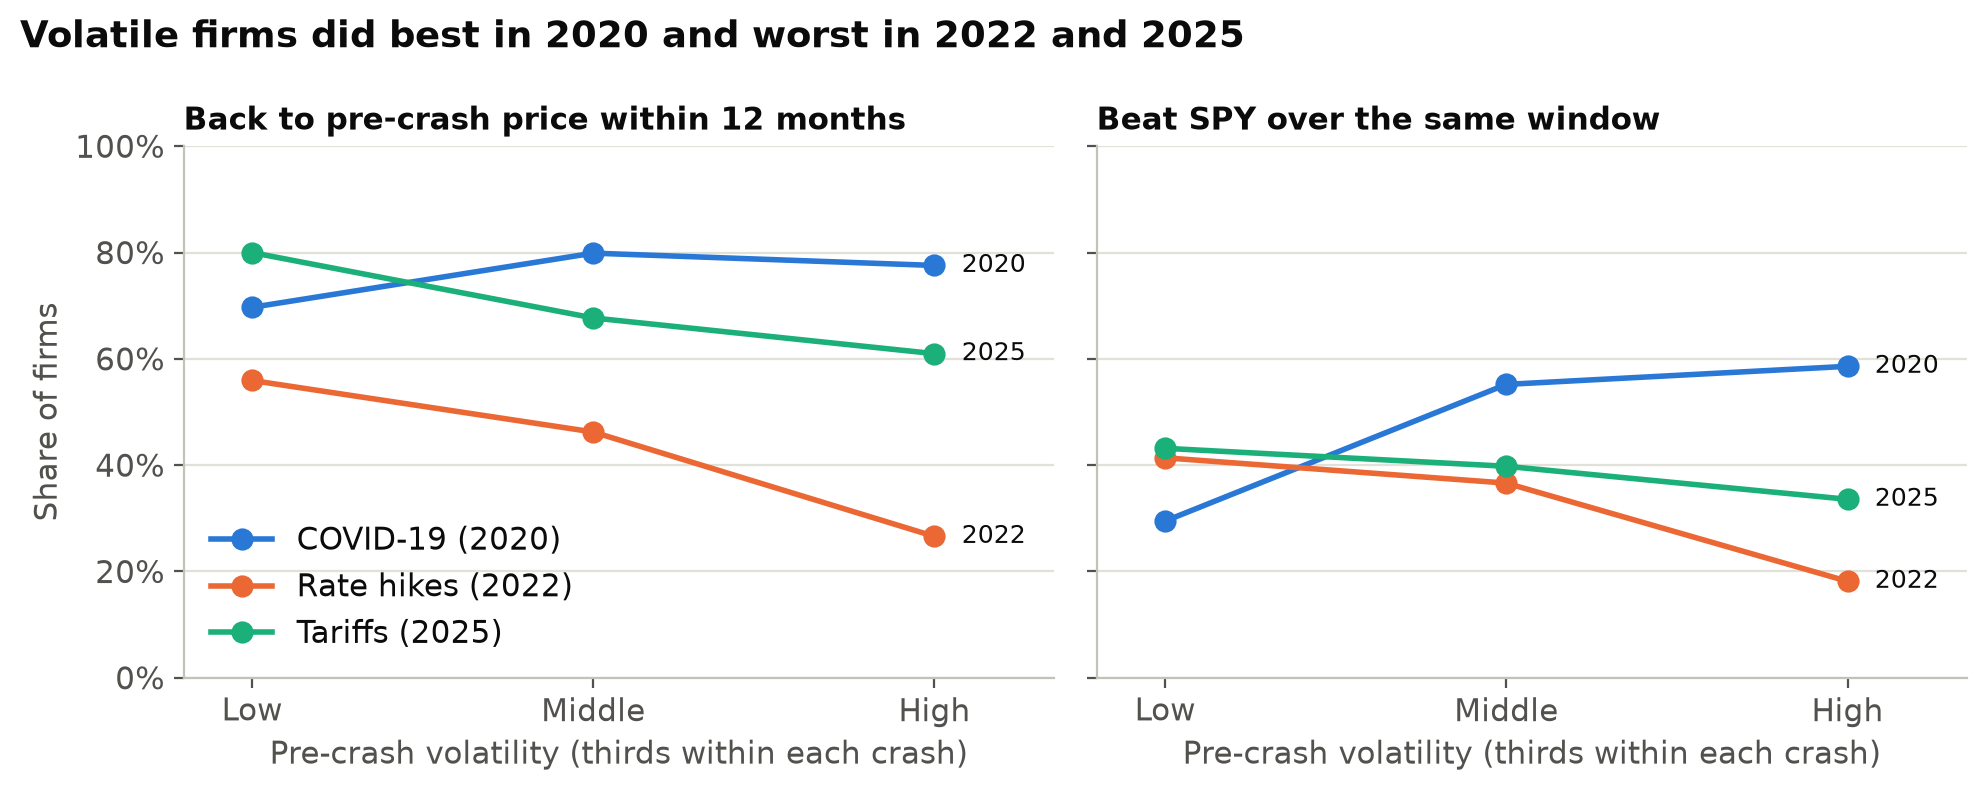
\includegraphics[width=0.85\textwidth]{volatility_flip.png}
\caption{Share of firms that recovered (left) and beat SPY (right), by pre-crash volatility third within each crash.}
\label{fig:flip}
\end{figure}

\subsection{Archetypes, rules, and exceptions}
\begin{itemize}
  \item \textbf{Archetypes.} k-means finds three broad archetypes ($k=3$, silhouette 0.15, adjusted Rand index of 0.999 across seeds). HDBSCAN labels 77\% of firms as noise, so these are broad tendencies, not tight groups.
  \item \textbf{The best archetype changes with the crash.} Profitable, cash-generating firms recovered most in 2020 (81\%). Large, calm firms led in 2022 (54\%) and 2025 (76\%). Loss-making firms fell furthest behind in 2022 (27\%).
  \item \textbf{Chi-square tests.} Recovery differs by archetype in every crash (Cram\'er's V 0.10 to 0.23). Each archetype's recovery rate differs across crashes (V 0.21 to 0.41), while the archetype mix barely changes (V 0.02).
  \item \textbf{Rules.} FP-Growth finds 91, 640, and 326 rules (support 5\%, lift at least 1.1). Few hold in all three crashes. The not-recovered rules from 2020 (low beta, low volatility, financial firms) reverse in 2022 and 2025.
  \item \textbf{Exceptions.} Isolation Forest flags 211 unusual rows. They recovered less often (49\% vs 63\%), and 13\% of them had a price move of more than 3x. LOF barely agrees with it (Jaccard 0.08).
\end{itemize}

\subsection{Timing}
\begin{itemize}
  \item \textbf{Recovery by crash.} By 18 months, Kaplan--Meier estimates that 84\%, 50\%, and 77\% of firms had recovered. Median days to recovery were 247, 539, and 142.
  \item \textbf{Failures} were rare (0.4 to 0.8\% within 12 months), so treating them as a competing risk changes nothing.
  \item \textbf{Cox model.} Concordance is 0.61, 0.65, and 0.58 by crash. Momentum is the only feature that is significant with the same sign in all three crashes (hazard ratio 1.07 to 1.09). Return on assets, size, beta, and being a financial firm change sign across crashes.
  \item \textbf{Assumption check.} The proportional-hazards check fails for some features, so these hazard ratios are averages over time.
\end{itemize}

\subsection{Robustness}
The gap between within-crash and cross-crash AUC survives every check we tried (Table~\ref{tab:robust}).

\begin{table}[h]
\centering\small
\caption{Robustness checks (LightGBM; mean AUC for recovery unless noted).}
\label{tab:robust}
\begin{tabularx}{\textwidth}{Xcc}
\toprule
Check & Within crash & Across crashes \\
\midrule
Main result & 0.69 & 0.51 \\
Drop the 377 firms acquired before 12 months & 0.690 & 0.510 \\
Beta-adjusted label (beat beta $\times$ SPY return) & 0.702 & 0.480 \\
Within-crash percentiles instead of raw features & -- & change of $-0.004$ \\
Firms seen in training vs firms not seen & -- & same pattern \\
Yahoo prices only & within $\pm 0.04$ & about 0.5 \\
Peak-day close as the pre-crash price & same pattern & same pattern \\
\bottomrule
\end{tabularx}
\end{table}

% ---------------- 6. Conclusions ----------------
\section{Conclusions and future work}

Pre-crash fundamentals do predict which firms recover, but only within the crash a model was trained on. Across crashes, the same models do worse than a baseline that only knows sector and size, because signals change sign with the crash's cause. Volatility helped in the 2020 liquidity panic and hurt in the 2022 rate shock and the 2025 tariff shock. Almost no signal is universal. For practice, a ``crash-resilient'' stock screen built on one crash should not be trusted in the next unless that crash had a similar cause.

\textbf{Limits.}
\begin{itemize}
  \item With only three crashes, the link to crash type is an interpretation; it cannot be modeled directly.
  \item 3.4\% of matched rows have no checked price. They are smaller and fail more often, so some survivorship bias remains, mostly in 2020.
  \item 7.5\% of rows could not be identity-checked, because they have no fails record at the peak.
  \item Prices come from two sources, although results hold with Yahoo alone.
  \item SIC codes are current, not as of each crash.
  \item The archetype structure is weak, and the proportional-hazards assumption fails for some features.
\end{itemize}

\textbf{Future work.}
\begin{itemize}
  \item Add more crashes (2008, 2011, 2018), so that crash type could become a model input.
  \item Use market conditions before a crash to choose which past crash to learn from.
  \item Test models whose signals are allowed to change with interest rates or volatility.
\end{itemize}

% ---------------- References ----------------
\begin{thebibliography}{99}
\small
\bibitem{breiman2001} L.~Breiman. Random forests. \emph{Machine Learning}, 45(1):5--32, 2001.
\bibitem{breunig2000} M.~M. Breunig, H.-P. Kriegel, R.~T. Ng, and J.~Sander. LOF: Identifying density-based local outliers. In \emph{Proc.\ ACM SIGMOD}, pages 93--104, 2000.
\bibitem{campello2013} R.~J. G.~B. Campello, D.~Moulavi, and J.~Sander. Density-based clustering based on hierarchical density estimates. In \emph{Proc.\ PAKDD}, pages 160--172, 2013.
\bibitem{cox1972} D.~R. Cox. Regression models and life-tables. \emph{Journal of the Royal Statistical Society, Series B}, 34(2):187--220, 1972.
\bibitem{delong1988} E.~R. DeLong, D.~M. DeLong, and D.~L. Clarke-Pearson. Comparing the areas under two or more correlated receiver operating characteristic curves: A nonparametric approach. \emph{Biometrics}, 44(3):837--845, 1988.
\bibitem{ding2021} W.~Ding, R.~Levine, C.~Lin, and W.~Xie. Corporate immunity to the COVID-19 pandemic. \emph{Journal of Financial Economics}, 141(2):802--830, 2021.
\bibitem{fahlenbrach2021} R.~Fahlenbrach, K.~Rageth, and R.~M. Stulz. How valuable is financial flexibility when revenue stops? Evidence from the COVID-19 crisis. \emph{Review of Financial Studies}, 34(11):5474--5521, 2021.
\bibitem{fred} Federal Reserve Bank of St.~Louis. Federal Reserve Economic Data (FRED): SP500, VIXCLS, DGS10. \url{https://fred.stlouisfed.org/}.
\bibitem{gu2020} S.~Gu, B.~Kelly, and D.~Xiu. Empirical asset pricing via machine learning. \emph{Review of Financial Studies}, 33(5):2223--2273, 2020.
\bibitem{han2000} J.~Han, J.~Pei, and Y.~Yin. Mining frequent patterns without candidate generation. In \emph{Proc.\ ACM SIGMOD}, pages 1--12, 2000.
\bibitem{holm1979} S.~Holm. A simple sequentially rejective multiple test procedure. \emph{Scandinavian Journal of Statistics}, 6(2):65--70, 1979.
\bibitem{kaplan1958} E.~L. Kaplan and P.~Meier. Nonparametric estimation from incomplete observations. \emph{Journal of the American Statistical Association}, 53(282):457--481, 1958.
\bibitem{ke2017} G.~Ke, Q.~Meng, T.~Finley, T.~Wang, W.~Chen, W.~Ma, Q.~Ye, and T.-Y. Liu. LightGBM: A highly efficient gradient boosting decision tree. In \emph{Advances in Neural Information Processing Systems 30}, 2017.
\bibitem{liu2008} F.~T. Liu, K.~M. Ting, and Z.-H. Zhou. Isolation forest. In \emph{Proc.\ IEEE ICDM}, pages 413--422, 2008.
\bibitem{lundberg2017} S.~M. Lundberg and S.-I. Lee. A unified approach to interpreting model predictions. In \emph{Advances in Neural Information Processing Systems 30}, 2017.
\bibitem{ramelli2020} S.~Ramelli and A.~F. Wagner. Feverish stock price reactions to COVID-19. \emph{Review of Corporate Finance Studies}, 9(3):622--655, 2020.
\bibitem{secapi} U.S. Securities and Exchange Commission. EDGAR application programming interfaces (XBRL company facts and submissions). \url{https://www.sec.gov/search-filings/edgar-application-programming-interfaces}.
\bibitem{secftd} U.S. Securities and Exchange Commission. Fails-to-deliver data. \url{https://www.sec.gov/data-research/sec-markets-data/fails-deliver-data}.
\bibitem{sun2014} X.~Sun and W.~Xu. Fast implementation of DeLong's algorithm for comparing the areas under correlated receiver operating characteristic curves. \emph{IEEE Signal Processing Letters}, 21(11):1389--1393, 2014.
\bibitem{tiingo} Tiingo. End-of-day stock price API. \url{https://www.tiingo.com/documentation/end-of-day}.
\bibitem{yfinance} R.~Aroussi. yfinance: Download market data from Yahoo! Finance's API. \url{https://github.com/ranaroussi/yfinance}.
\end{thebibliography}

\end{document}
